\documentclass[a4paper,12pt]{article}

\usepackage{latexsym}
\usepackage[utf8]{inputenc}
\usepackage[T1]{fontenc}
\usepackage{graphicx}
\usepackage{amsmath}
\usepackage{float}% If comment this, figure moves to Page 2
\usepackage{hyperref}
\usepackage{lipsum}

\author{Krzysztof~Palka and Dominik~Odrowski}
\date{April 18, 2013}

\title{\textsc{Exercise} 418 \\ Measurement of the speed of light} 

\addtolength{\textwidth}{2.5cm}
\addtolength{\hoffset}{-1.25cm}

\begin{document}

    \maketitle

    \begin{abstract}
        This report presents measurement of the speed of light in air, in liquid and calculation of index of refraction for this liquid based phase shift of light wave.
    \end{abstract}

    \section{Introduction}
    The aim of this exercise was to determine, using modulated light and basing on phase shift of wave, the speed of light in the vacuum. Then, using vessel field with liquid, determination of index of refraction and speed of light for this liquid.   

    \section{Theory and measurement}
    Measurement base on determination of time in which light covers the relatively small distance (couple of meters). Because it is very difficult to measure that time, which is very short, so we had to use indirect method.
    As source of light we used diode which send modulated light (light with constant frequency) which was equal approximately 50 MHz. Light traveled distance L form diode to mirrors which reflects it and sends to receiver located next to source. Both source and receiver are connected with oscilloscope. We could presets wave of light as 2 sinusoids or set input from source on OX and input from receiver on OY. Hence the aim was to determine phase shift, we have chosen second option, because we was interested only in finding phase shift equal to $\pi$ or $2 \pi$. When waves were in the same phase, or their phases were shifted by $\pi$, then the plot with XY oscilloscope's mode looked like straight line. For those phases obtained lines are called Lissajous curves.
    Knowing distance in which there is phase shift, which is multiplication of $\pi$ by $N$, where $N$ is natural number we are able, basing of knowledge of wave behavior, determine speed of light from equation (in this case for phase shift equal to $\pi$):
    \begin{equation}
        c = 4 f (x_B - x_A) \label{eq:c}
    \end{equation}
    where $f$ is frequency of send light and $x_A$ and $x_B$ are distances of displacement of mirror, for which phase shifts were equals 0 and $\pm \pi$ 

    \begin{figure}[H]
    \begin{center}
        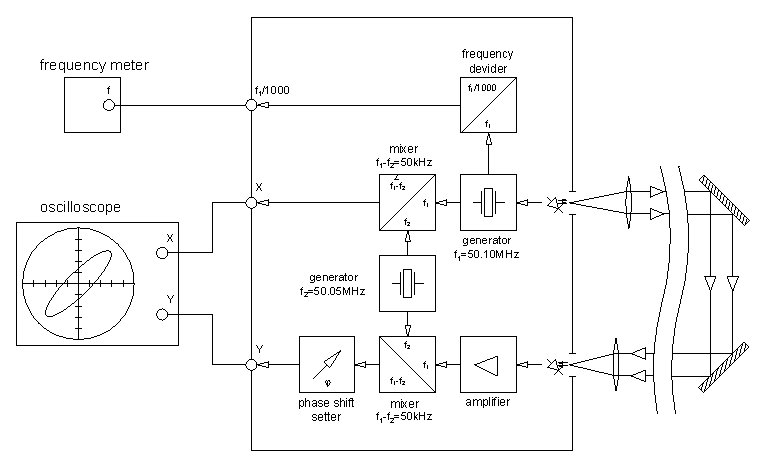
\includegraphics[width=0.9\textwidth]{set-up}
        \caption{Diagram of experimental set-up \cite{E418}.}
        \label{fig:set-up}
    \end{center}
    \end{figure}

    In similar way we can determinate speed of light $v$ in liquid. To do this we can put vessel with liquid on path of the light, and then relying on previous description and knowing length of vessel $L_0$ we can determine speed of light. Moreover, basing on dependency $v = c/n$ \cite{HRW} we can determine index of refraction $n$ for this liquid. For further calculation we will use equation for $n$ and $v$ in following form:

    \begin{equation}
        n = 2 \frac{x_2-x_1}{L_0} + 1 \label{eq:n}
    \end{equation}
    
    \begin{equation}
        v = \frac{L_0 c}{2(x_2 - x_1) + L_0} \label{eq:v}
    \end{equation}
    where $x_2$ and $x_1$ are distances of displacement of mirror, for which phase shifts were equals 0 and $\pm \pi$ 


    \section{Results}
    
    The speed of light in the air is calculated form equation \ref{eq:c}. First we had to calculate distance $ d = |x_B - x_A|$ and then substitute it to equation. 

    \begin{table}[h]
        \begin{center}
            \caption{Measured distances $x_A$, $x_B$ and calculated displacement and the speed of light in air}
            \label{tab:c}
            \begin{tabular}{|c|c|c|c|}
                \hline
                $x_A$ [$10^{-2}$ m] & $x_B$ [$10^{-2}$ m] & $d$ [$10^{-2}$ m] & $c$ [$10^8 \frac{\mathrm m}{\mathrm s}$] \\ 
                \hline
                18.7 & 168.7 & 150.0 & 3.000\\
                23.7 & 172.7 & 149.0 & 2.980\\
                28.7 & 177.8 & 149.1 & 2.982\\
                33.7 & 182.5 & 148.8 & 2.976\\
                38.7 & 187.7 & 149.0 & 2.980\\
                \hline
            \end{tabular}
        \end{center}
    \end{table}

    The resolution of meter is $\pm 0.1$ cm, so we can calculate how this affect results.
    \begin{equation}
        \Delta c = \left| \frac{c(d)}{\mathrm{d} d}\right| \cdot \Delta d = 4 f \cdot \Delta d
    \end{equation}
    \begin{displaymath}
        \Delta c = 4 \cdot 50 \cdot 10^6 \frac{1}{\mathrm{s}} \cdot 10^{-3} \mathrm{m} = 0.002 \cdot 10^8 \frac{\mathrm{m}}{\mathrm{s}}
    \end{displaymath}

    So it is obvious that $\Delta d$ is not a resolution of meter and it is much bigger than 0.1~cm. Therefore there is no point of calculating error for that vale. We have included more information about that in conclusions. But we can calculate average value for~$c$, as uncertainty we used margin of error form Student's $t$-test with 95\% confidence interval.

    \begin{displaymath}
        c = (2.99\pm0.02) \cdot 10^8 \frac{\mathrm m}{\mathrm s}
    \end{displaymath}
    
    Now we will present results of measurements needed to calculate speed of light in liquid and index of refraction for that liquid. We used equations \ref{eq:v} and \ref{eq:n}. As there are 2 possible displacements which gives us desirable phase shift, so we have labeled them as $d_1$ which is $x_B - x_D$ and $d_2$---$x_C - x_E$. Of course their are substituted to $x_2 - x_1$ values form equations.   
    Length of vessel with liquid was 1 m. 


    \begin{table}[H]
        \begin{center}
            \caption{Measured distances $x_A$, $x_B$, $x_C$, $x_D$, $x_E$, calculated speed of light in liquid and index of refraction for displacement $d_1$ and $d_2$}
            \label{tab:vn}
            \begin{tabular}{|c|c|c|c|c|c|c|c|c|}
                \hline
                $x_A$ [cm] & $x_B$ [cm] & $x_C$ [cm] & 
                $x_D$ [cm] & $x_E$ [cm] & 
                $v_1$ [$10^8 \frac{\mathrm m}{\mathrm s}$] &
                $v_2$ [$10^8 \frac{\mathrm m}{\mathrm s}$] &
                $n_1$ & $n_2$ \\ 
                \hline
                12.8 & 161.7 & 314.3 & 141.0 & 296.7 & 2.122 & 2.219 & 1.414 & 1.352\\
                17.8 & 167.7 & 320.0 & 148.9 & 303.9 & 2.180 & 2.269 & 1.376 & 1.322\\
                22.8 & 171.3 & 322.6 & 154.2 & 316.0 & 2.235 & 2.650 & 1.342 & 1.132\\
                27.8 & 176.5 & 331.8 & 158.3 & 339.6 & 2.199 & 3.555 & 1.364 & 0.844\\
                \hline
            \end{tabular}
        \end{center}
    \end{table}

    As we can see inconsistency of values $v_2$ and $n_2$ which were calculated basing on $d_2$ is bigger than those measured for $d_1$ which leads us to another concussion causes to skip those values. So the average values of $v$ and $n$ ($v_1$ and $n_1$) with margin of error form Student's $t$-test with 95\% confidence interval treated as uncertainty are as following. 

    \begin{displaymath}
        v = (2.19 \pm 0.07) \cdot 10^8 \frac{\mathrm m}{\mathrm s}
    \end{displaymath}
    
    \begin{displaymath}
        n = 1.37 \pm 0.05
    \end{displaymath}

    \section{Conclusions}
    As we have seen treating resolution of meter as uncertainty was not sufficient method. It was because there was much wider range of values that we could read when it seemed that we have seen straight line, not elips. It [$\Delta d$] could be not even counted in millimeters but in centimeters, so it has huge influence on results. If we compare obtained speed of the light in the air to values from literature $c = 2.998 \cdot 10^8 \frac{\mathrm m}{\mathrm s}$) then we see it is within boundary of error. What is interesting, if light traveled longer distance results were less accurate because of previously mansion reason. Apparently $\Delta d$ is bigger if distance traveled by light increases. We see it in measurement of speed of light in liquid. It led us to skip results obtained for the longest distances. If we compare results of speed of light with literature, we see that their are similar to those for water ($v = 2.254 \cdot 10^8 \frac{\mathrm m}{\mathrm s}$). Index of refraction 1.33---which is---for water is also within boundary of error, but the uncertainty obtained form student's $t$-test is quite big.  It could be caused by the fact, that we haven't considered glass of which vessel is build and air, through which light comes. Applying this factors can give more accurate results.     

    

    \begin{thebibliography}{9}
        \bibitem{E418}\emph{Ćwiczenie 418. Pomiar prędkości światła} [online]. Pracownia Fizyki Współczesnej Instytutu Fizyki PŁ. Łódź. Available online at: \url{http://phys.p.lodz.pl/materialy/mdems/418 (pl).pdf}. Accessed April 23, 2013.
        \bibitem{HRW}\emph{Fundamentals of physics} (2011) [ebook]. David Halliday, Robert Resnick, Jearl Walker. 9th ed. ISBN 978-0-470-46908-8
    \end{thebibliography}

\end{document}
